\documentclass{beamer}
\usepackage{listings}
\usepackage{color}
\usepackage{amsmath}
\usepackage{gvv}

\title{System of Equations}
\author{EE25BTECH11008 - Anirudh M Abhilash}
\date{October 4, 2025}

\begin{document}

%----------------- Title -------------------
\begin{frame}
\titlepage
\end{frame}

%----------------- Problem -------------------
\begin{frame}{Problem Statement}
Solve the following system of equations:
\begin{align*}
x - y = 8, \\ 3x - 3y = 16
\end{align*}
\end{frame}

%----------------- Solution -------------------
\begin{frame}{Solution}
Each equation can be expressed in vector form as a dot product:
\begin{align}
\myvec{1 & -1}\myvec{x \\ y} &= 8, \\
\myvec{3 & -3}\myvec{x \\ y} &= 16.
\end{align}

Stacking these gives the matrix equation
\begin{align}
\myvec{1 & -1 \\ 3 & -3}\myvec{x \\ y} &= \myvec{8 \\ 16}.
\end{align}
\end{frame}

%----------------- Solution (cont) -------------------
\begin{frame}{Solution (cont..)}
In augmented form,
\begin{align}
\augvec{2}{1}{1 & -1 & 8 \\ 3 & -3 & 16}.
\end{align}

Applying the row operation $R_2 \to R_2 - 3R_1$,
\begin{align}
\augvec{2}{1}{1 & -1 & 8 \\ 0 & 0 & -8}.
\end{align}

This yields the contradiction
\begin{align}
0 = -8.
\end{align}
Hence the system is inconsistent,
\[
\boxed{\text{No solution}}
\]

\end{frame}

\begin{frame}[fragile]{Python Code (Plotting Line and Vectors)}
\begin{lstlisting}[language=Python]
import numpy as np
import matplotlib.pyplot as plt

x = np.linspace(-5, 15, 400)
y1 = x - 8
y2 = x - 16/3

plt.figure(figsize=(8, 6))
plt.plot(x, y1, color='blue')
plt.plot(x, y2, color='red')
plt.text(10, 2, r'$x - y = 8$', color='blue', fontsize=12)
plt.text(10, 7, r'$3x - 3y = 16$', color='red', fontsize=12)

\end{lstlisting}
\end{frame}

\begin{frame}[fragile]{Python Code (cont..)}
\begin{lstlisting}[language=Python]
plt.title("Plot of the system of equations")
plt.xlabel("x")
plt.ylabel("y")
plt.grid(True)
plt.axhline(0, color='black', linewidth=0.5)
plt.axvline(0, color='black', linewidth=0.5)

plt.show()
\end{lstlisting}
\end{frame}

%----------------- Plot -------------------
\begin{frame}[fragile]{Plot}
\begin{figure}[H]\centering
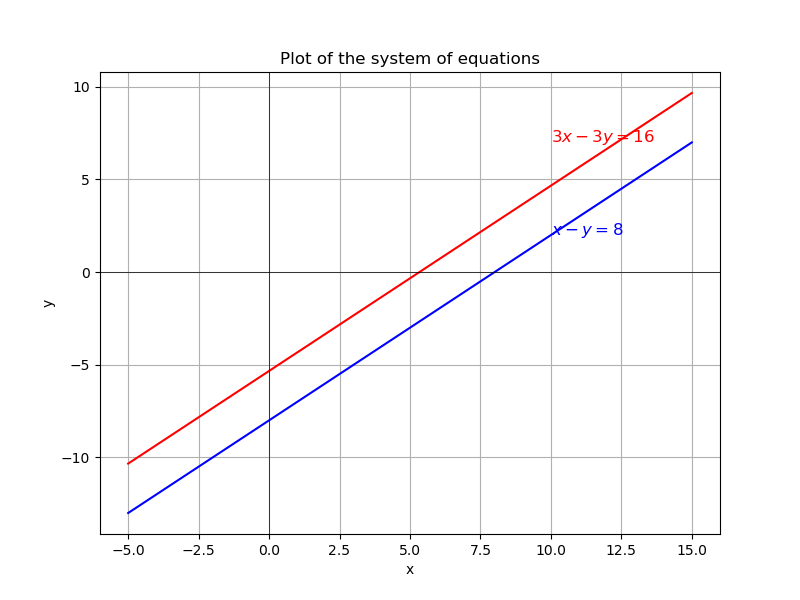
\includegraphics[width=0.8\columnwidth]{figs/plt.png}
\caption{System of Equations}
\label{fig:plt}
\end{figure}
\end{frame}

%----------------- C Code -------------------

\begin{frame}[fragile]{C Code (Computations)}
\begin{lstlisting}[language=C]
#include <stdio.h>

void get_lines(double* x, double* y1, double* y2, int n) {
    for (int i = 0; i < n; i++) {
        y1[i] = x[i] - 8; 
        y2[i] = x[i] - 16.0/3.0; 
    }
}
\end{lstlisting}
\end{frame}

%----------------- Python Code -------------------
\begin{frame}[fragile]{Python Code (Using C)}
\begin{lstlisting}[language=Python]
import numpy as np
import matplotlib.pyplot as plt
import ctypes

lines_lib = ctypes.CDLL('./points.so')

n = 100
x = np.linspace(-5, 15, n)
y1 = np.zeros(n, dtype=np.float64)
y2 = np.zeros(n, dtype=np.float64)
\end{lstlisting}
\end{frame}

\begin{frame}[fragile]{Python Code (Cont..}
\begin{lstlisting}[language=Python]
lines_lib.get_lines.argtypes = [
    np.ctypeslib.ndpointer(dtype=np.float64, ndim=1, flags="C_CONTIGUOUS"),
    np.ctypeslib.ndpointer(dtype=np.float64, ndim=1, flags="C_CONTIGUOUS"),
    np.ctypeslib.ndpointer(dtype=np.float64, ndim=1, flags="C_CONTIGUOUS"),
    ctypes.c_int
]
lines_lib.get_lines(x, y1, y2, n)

plt.figure(figsize=(8, 6))
plt.plot(x, y1, color='blue')
plt.plot(x, y2, color='red')
\end{lstlisting}
\end{frame}

\begin{frame}[fragile]{Python Code (Cont..)}
\begin{lstlisting}[language=Python]
plt.text(10, 2, r'$x - y = 8$', color='blue', fontsize=12)
plt.text(10, 7, r'$3x - 3y = 16$', color='red', fontsize=12)

plt.title("System of Equations")
plt.xlabel("x")
plt.ylabel("y")
plt.grid(True)
plt.axhline(0, color='black', linewidth=0.5)
plt.axvline(0, color='black', linewidth=0.5)
plt.show()
\end{lstlisting}
\end{frame}

\end{document}